\section{Measure Theory and Integration}
\subsection{Measure Space}
In the normal sense of the word ``measure'', the measure of any interval $I=[a,b]$, in $\RR$ coincides with the length $\ell(I)=|b-a|$. Similarly, the area of a square $S = [a_1,b_1]\times [a_2,b_2] = I_1\times I_2$ in $\RR^2$ is $\ell(I_1)\cdot\ell(I_2)$. More generally, given intervals $I_k = [a_k,b_k], k = 1,\ldots, n$, the volume of the box $B= I_1\times \ldots \times I_n$ in  $\RR^n$ is $\prod\limits_{k=1}^n \ell(I_k)$. Measure theory generalizes the length, area and volume to other measures on other abstract sets $\Omega$ rather than $\RR^n$. Moreover, this branch of real analysis establishes the class of measurable subsets of $\Omega$. To see the reason for this diligent work of mathematicians on measure theory, let us take an example on the measure of length. As in ordinary contexts, the length $\ell(E)$ of any subset $E$ of $\RR$, if exists, is required to satisfy

\begin{enumerate}
 \item Non-negativity: $\ell(E) \ge 0$.
 \item If $E\subset F\subset \RR$, then $\ell(E)\le \ell(F)$.
 \item If $E=[a,b]$, then $\ell(E) = |b-a|$.
 \item Translation invariance: for any $x\in\RR$, $\ell(E+x) = \ell(E)$.
 \item If $E$ can be divided to a collection of disjoint intervals $\{I_k\}_{k\in N}$, assuming that $\ell(\varnothing) = 0$, then $\ell(E) = \sum\limits_{k=1}^\infty \ell(I_k).$
\end{enumerate}

We will prove that our intuitive length measure cannot be applied for all subsets of $\RR$ \cite{vitali1905sul}.

\begin{proposition}
 If there exists $\ell : 2^\RR \to [0,\infty]$ satisfying
 \begin{enumerate}[label=(\arabic*)]
  \item If $E=[a,b]$, then $\ell(E) = |b-a|$. Also assume that $\ell(\varnothing) = 0$.
  \item If $E\subset F\subset \RR$, then $\ell(E)\le \ell(F)$.
  \item Translation invariance: for any $x\in\RR$, $\ell(E+x) = \ell(E)$.
  \item If $E$ can be divided to a collection of disjoint intervals $\{I_k\}_{k\in N}$, then $\ell(E) = \sum\limits_{k=1}^\infty \ell(I_k).$
        % \item (Derived from (2) and (4)) for any collection  measurable sets $\{A_k\}_{k=1}^{\infty}$,
        %       $$\ell\left(\bigcup\limits_{k=1}^{\infty} A_k\right) \le \sum_{k=1}^{\infty} A_k.$$
 \end{enumerate}
 Then $\ell(E) = 0, \forall E\in 2^\RR$.
\end{proposition}

\begin{proof}
 By (2), we have $\ell((0,1])\le \ell([0,1]) = 1$. Let us define an equivalence relation \index{equivalence relation} on $(0,1]$ as
 $$x\sim y \Leftrightarrow x-y\in\QQ.$$
 Clearly, for any $x\in (0,1]$, we have the equivalence class
 $$[x] = \{y\in(0,1] : x-y\in \QQ\} = \{x+q: q\in \QQ, x+q\in (0,1]\}.$$
 Denote by $N\in\NN\cup\{\infty\}$ the number of equivalence classes. Choose an element $x_n$ from the $n$-th equivalence class, where $1\le n\le N$\footnote{We have made use of the Axiom of Choice}. Clearly all the $x_n, n\in1,\ldots, N$ are distinct.

 Let $A=\{x_k\}_{k=1}^N\subset(0,1]$ and $(q_n)_{n=1}^\infty$ be a numeration of $\QQ\cap(-1,1]$\footnote{The set of rational number $\QQ$ is countable}. Also, let $A_n = A + q_n$ for any $n\in\NN$. We claim that if $n\neq m$, then $A_n\cap A_m = \varnothing$. We will prove the contrapositive statement. Suppose that there exists $x\in A_n\cap A_m$, then $x=a_n + q_n = a_m + q_m$, where $a_n\in A_n$ and $a_m\in A_m$. Therefore,
 $$a_n-a_m = q_m-q_n\in \QQ,$$
 which implies that $a_n\sim a_m$. Hence, $a_n$ and $a_m$ are presentations of a single equivalent class, or $n=m$.

 On the other hand, $(0,1] \subset \bigcup\limits_{n=1}^\infty A_n \subset (-1,2]$.

 By (3) and (4),
 $$\ell((-1,2]) = \ell((-1,0]) + \ell((0,1]), \ell((1,2]) = 3\ell((0,1]).$$

 By (3), we have

 $$\ell(A_n) = \ell (A), \forall n\in\NN.$$

 By (4) and the previous implications,
 $$\ell((0,1]) \le \ell\left(\bigcup\limits_{n=1}^\infty A_n\right) = \sum\limits_{k=1}^{\infty} \ell(A_k) = \sum_{k=1}^{\infty} \ell(A) \le 3\ell((0,1]).$$

 This implies $\ell(A)=0$, and also $\ell((0,1])=0$. Therefore,

 $$\ell(\RR) = \ell\left(\bigcup\limits_{m\in\ZZ}(m,m+1] \right) = \sum\limits_{m\in\ZZ} \ell((m,m+1])= \sum\limits_{m\in\ZZ} \ell((0,1]) = 0.$$

 Thus, $\ell$ coincides with the zero function. However, this measure of length is unavailing.
\end{proof}


A measure space is the initial model to measure theory. Consider the following real-life example.

\begin{example}
 A farmer has a rectangular land whose width and length are both $100\,m$. The coordinated representation of the land is $\Omega=[0,100]\times[0,100]$. The farmer allocates a region to build a warehouse, whose shape is not restricted to be a rectangle. To approximate the area of this region, the farmer divides it into disjoint rectangular subregions and sums of the areas.
\end{example}

A region is a set of $\Omega$. We know that maybe some subsets of $\Omega$ cannot be measured. Let $\F\subset2^\Omega$ be the family of all measurable subsets of $\Omega$. The area of whole land is known by the farmer i.e. $\Omega\in\F$. On the other hand, if we can measure the area of the warehouse, the rest region's area can also be measured. Motivated by the context, the set of measurable regions as above is defined formally as a $\sigma$-algebra, as below.

\begin{definition}
 \label{definition:sigma-algebra}
 Given a set $\Omega$. A collection of subsets $\F$ of $\Omega$ is called a \textbf{$\sigma$-algebra}\index{$\sigma$-algebra} if
 \begin{enumerate}
  \item $\varnothing, \Omega\in\F$;
  \item If $A\in\F$, then $A^c\in\F$;
  \item If $A_1,A_2,\ldots\in\F$, then $A_1\cup A_2\cup\ldots\in\F$.
 \end{enumerate}
 The pair $(\Omega, \F)$ is called a \textbf{measurable space}\index{measurable space}.
\end{definition}

Definition \ref{definition:sigma-algebra} models measurable objects to be a collection $\F$ of subsets of a given set $\Omega$. Before the definition of a measure, we consider some examples and analytically derived theorems.

\begin{example}
 \label{example:1}
 Given a set $\Omega$, then $\{\varnothing, \Omega\}$ and the power set $2^\Omega$ are two trivial $\sigma$-algebras. Let $\Omega=\{1,2,3\}$, the collection $\F=\{\varnothing,\Omega, \{1\}, \{2,3\}\}$ is a $\sigma$-algebra on $\Omega$.
\end{example}

\begin{proposition}
 Let $\{\F_\alpha\}_{\alpha\in I}$ be an arbitrary family of $\sigma$-algebras on $\Omega$. Then the intersection $\F=\bigcap\limits_{\alpha\in I}\F_\alpha$ is a $\sigma$-algebra.
\end{proposition}

\begin{proof}
 We will check that $\F$ three conditions for a $\sigma$-algebra.

 Since $\varnothing,\Omega\in\F_\alpha,\forall\alpha\in I$, we have $\varnothing,\Omega\in\bigcap\limits_{\alpha\in I}\F_\alpha$.

 If $A\in\bigcap\limits_{\alpha\in I}\F_\alpha$, then $A\in \F_\alpha,\forall\alpha\in I$, leading to $A^c\in \F_\alpha,\forall\alpha\in I$. Hence, $A^c\in\bigcap\limits_{\alpha\in I}\F_\alpha.$

 Finally, if $A_i\in\F_\alpha,\forall i\in\ZZ^+,\forall \alpha\in I$, then $\bigcup\limits_{i\in\ZZ^+}A_i\in\F_\alpha,\forall\alpha\in I$. Therefore,
 $\bigcup\limits_{i\in\ZZ^+}A_i\in\bigcap\limits_{\alpha\in I}\F_\alpha.$
\end{proof}

\begin{remark}
 The union of $\sigma$-algebras on $\Omega$ is not necessarily a $\sigma$-algebra. For example,
 $$\F_1=\{\varnothing,\Omega, \{1\}, \{2,3\}\} \text{ and } \F_2=\{\varnothing,\Omega, \{2\}, \{1,3\}\}$$
 are two $\sigma$-algebras on $\Omega=\{1,2,3\}$, but
 $$\F=\F_1\cup\F_2=\{\varnothing,\Omega,\{1\},\{2\},\{2,3\},\{1,3\}\}$$ is not, since $\{3\}=\{2,3\}\cap\{1,3\}\notin \F$.
\end{remark}

Having mentioned in Example \ref{example:1}, any collection $\C$ of subsets of $\Omega$, has a trivial $\sigma$-algebra $2^\Omega$ that contains $\C$ i.e. $\C\subset2^\Omega$. Therefore, there exists the smallest $\sigma$-algebra containing $\C$.

\begin{theorem}
 \label{theorem:generated-sigma-algebra}
 Given a set $\Omega$ and a collection of its subsets $\C$, there exists the smallest $\sigma$-algebra containing $\C$, denoted by $\sigma(\C)$, given by
 $$\sigma(\C)=\bigcap\limits_{\alpha\in I}\F_\alpha,$$
 where $\{\F_\alpha\}_{\alpha\in I}$ is the set of $\sigma$-algebras containing $\C$. We also called $\sigma(\C)$ to be the $\sigma$-algebra generated by $\C$.
\end{theorem}

\begin{proof}
 Since $\sigma(\C)$ itself is a $\sigma$-algebra containing $\C$ so $\sigma(\C)\in\{\F_\alpha\}$, leading to

 $$\bigcap\limits_{\alpha\in I}\F_\alpha\subset \sigma(\C).$$

 Moreover, $\bigcap\F_i$ is also a $\sigma$-algebra containing $\C$ and $\sigma(\C)$ is the smallest one, hence

 $$\sigma(\C)\subset\bigcap\limits_{\alpha\in I}\F_i.$$

 Thus, $\sigma(\C)=\bigcap\limits_{\alpha\in I}\F_i$.
\end{proof}

\begin{remark}
 Theorem \ref{theorem:generated-sigma-algebra} tells us that a collection of measurable subsets can be extended to a $\sigma$-algebra. For example, a collection $\C=\{\{1\}\}$ of subsets of $\Omega=\{1,2,3\}$ generates the $\sigma$-algebra
 $$\F=\{\varnothing,\Omega,\{1\},\{2,3\}\}.$$
\end{remark}

\begin{figure}[ht]
 \centering
 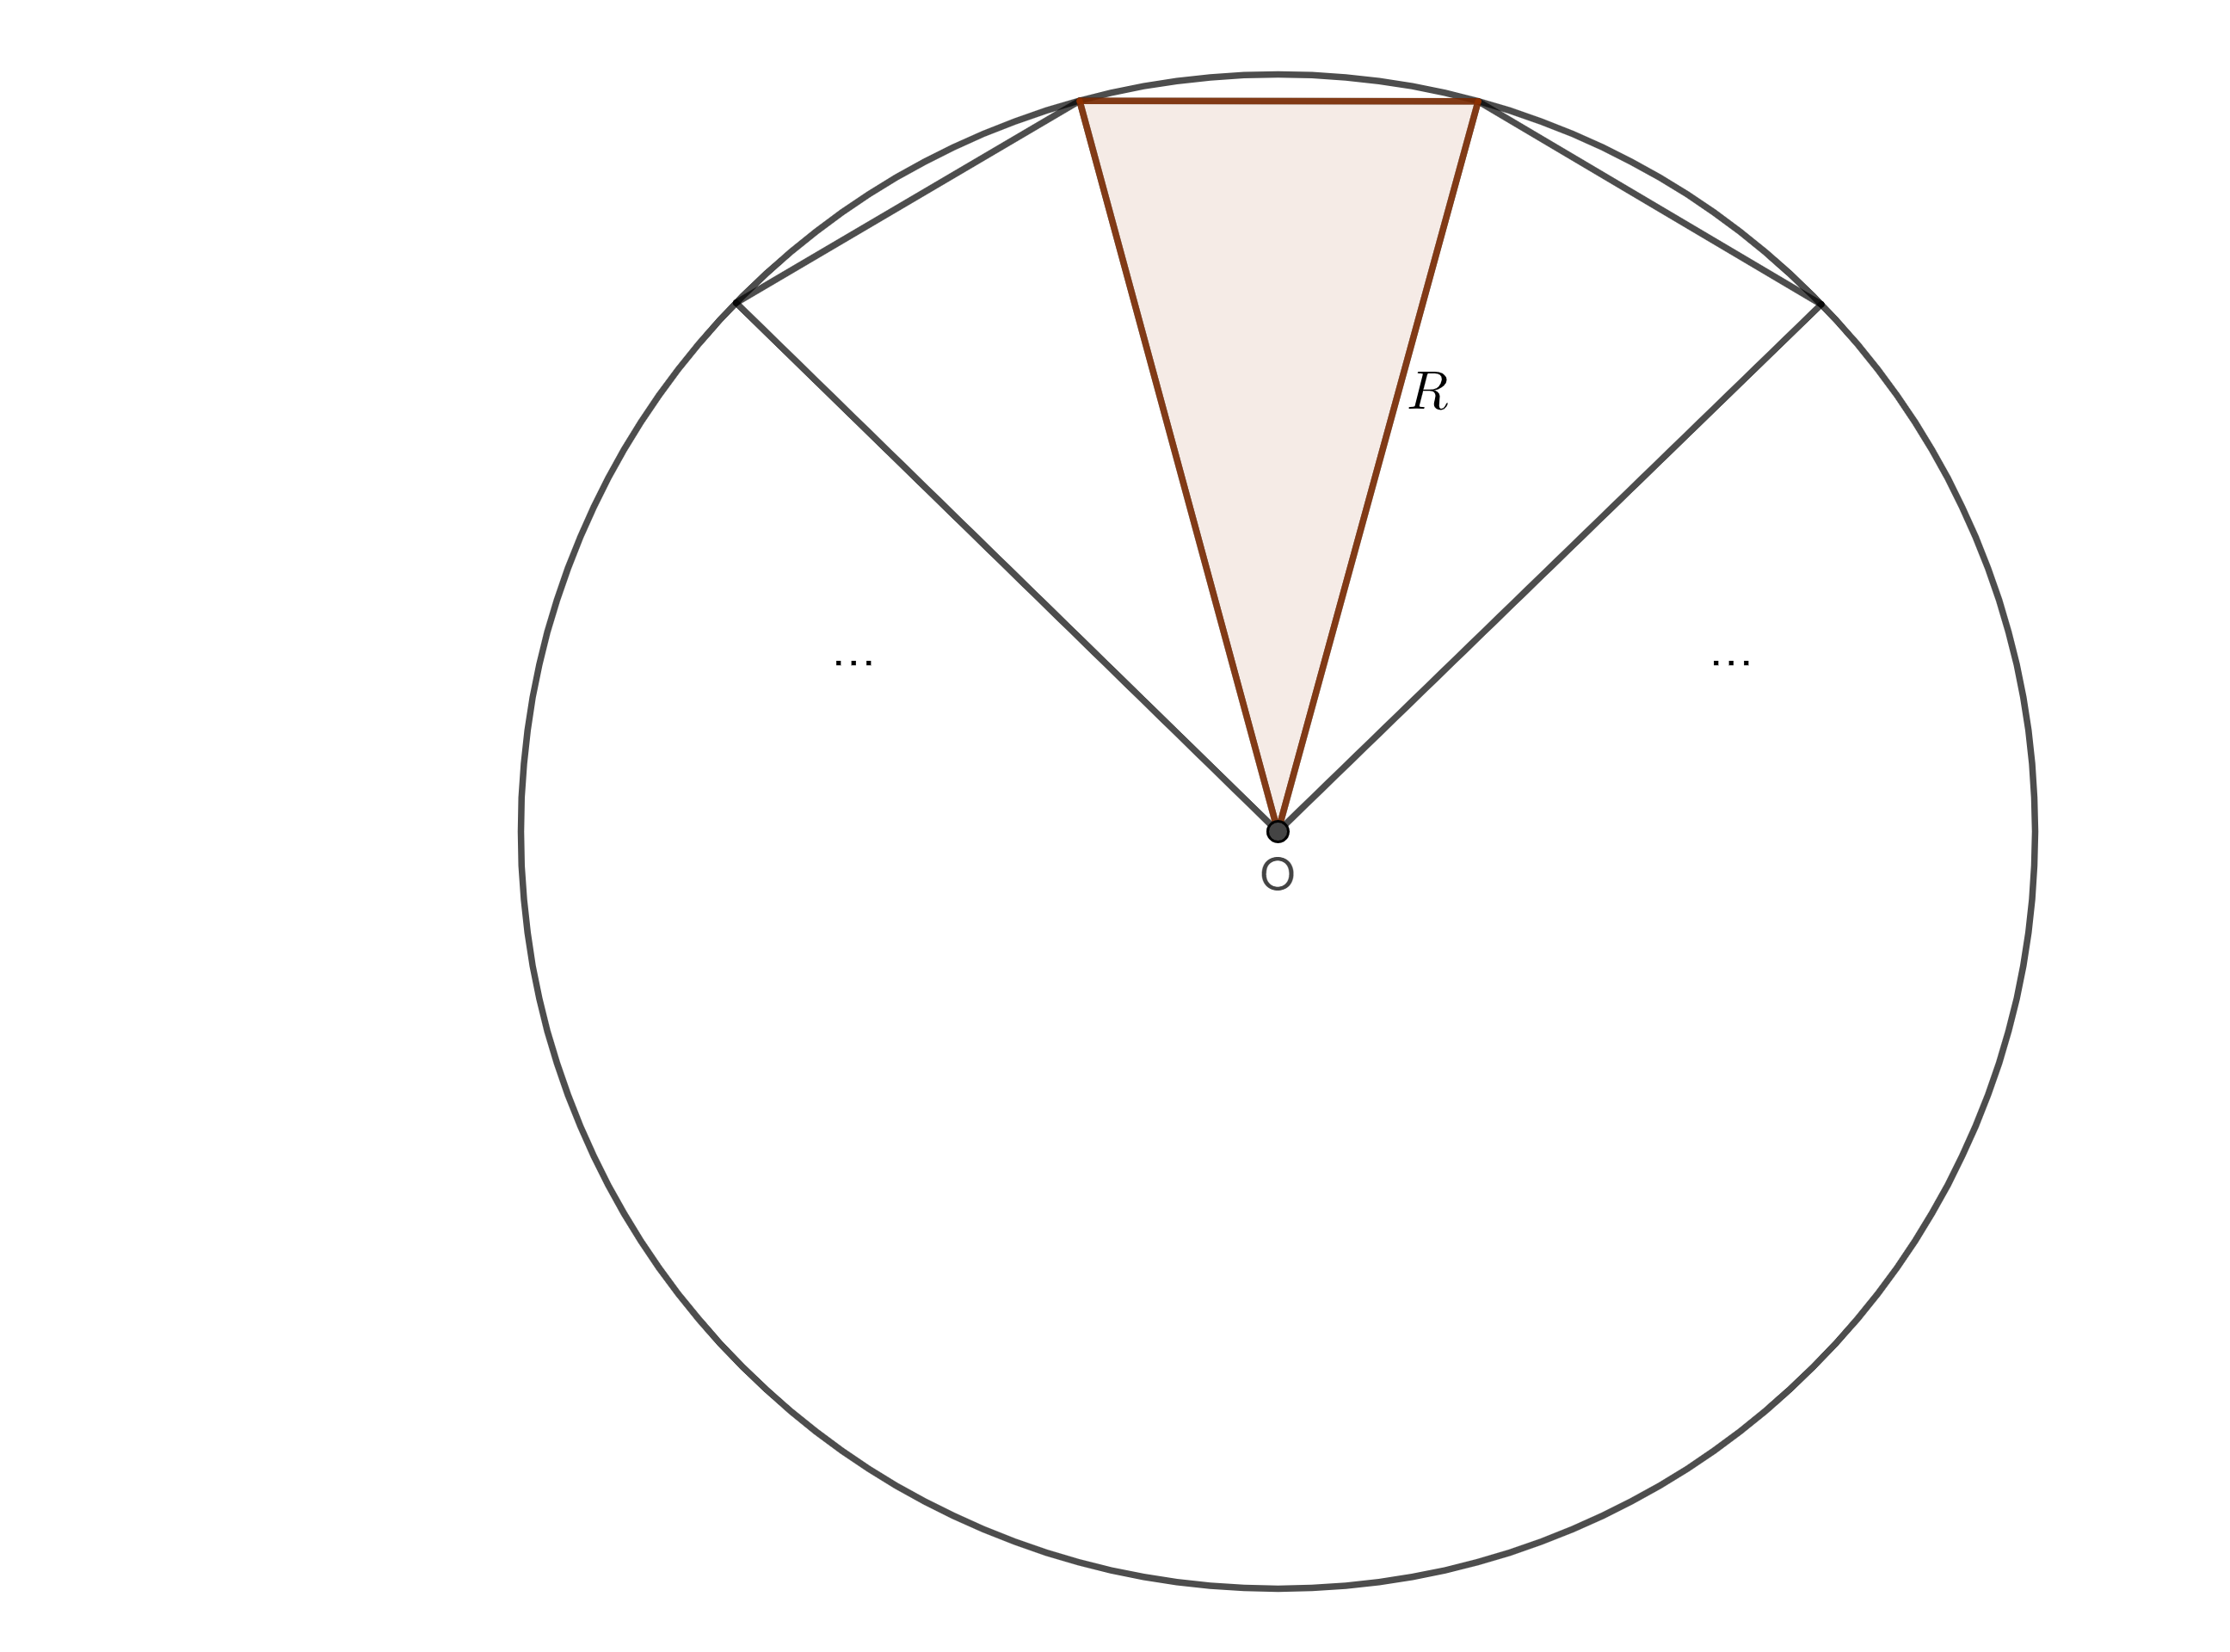
\includegraphics[width=0.4\linewidth]{img/circle.png}
 \vspace{0.5cm}
 \caption[Circle area approximation]{The area of a circle can be calculated by dividing it into equal isosceles triangles. As the number of triangles tends to infinity, the sum of bottom sides tends to the perimeter $2\pi R$ of the circle and the attitude of a triangle tends to $R$. Hence, the area is $A=\dfrac{1}{2}(2\pi R)R=\pi R^2$.}
 \label{figure:circle}
\end{figure}

\begin{definition}
 Given a measurable space $(\Omega,\F)$, a function $\mu:\F\to\RR$ is called a \textbf{measure}\index{measure} if it satisfies
 \begin{enumerate}
  \item Non-negativity: $\mu(A)\ge0,\forall A\in\F.$
  \item $\mu(\varnothing)=0$.
  \item Countable additivity: if $\{A_i\}_{i=1}^\infty\subset\F$ contains pairwise disjoint elements, then
        $$\mu\left(\bigcup\limits_{i=1}^\infty A_i\right)=\sum\limits_{i=1}^\infty \mu(A_i).$$
        The triplet $(\Omega,\F,\mu)$ is called a measure space.
 \end{enumerate}
\end{definition}

% \begin{theorem}[Properties of a measure]
%   \begin{enumerate}
%     \item[]
%     \item Monotonicity\index{monotonicity}: if $A\subset B$, then $\mu(A)\le\mu(B)$.
%   \end{enumerate}
% \end{theorem}

\begin{example}
 \begin{enumerate}
  \item []
  \item Consider the measurable space $(\RR, \B(\RR))  $. The function of taking the length of open intervals on the real line
        $$\mu((x,y))=|y-x|,\forall x,y\in\RR,$$
        which an assumption that $\mu(\varnothing)=0$, is a measure. Three properties of a measure are satisfied trivially.
  \item Consider the measurable space $(\RR, \F)$, where $\F$ is any $\sigma$-algebra on $\RR$. Given $a\in\RR$. The indicator function $\mathbf{1}_a: \F\to\{0,1\}$ given by
        $$\begin{cases}
          \mathbf{1}_a(X)=1, & \text{ if } a\in X \\
          \mathbf{1}_a(X)=0, & \text{ otherwise }
         \end{cases}$$
        is a measure. We already have $\mathbf{1}_a(X)\ge0, \forall a\in X$. Let us check the other two properties of a measure for this function.
        \begin{itemize}
         \item Since $a\notin\varnothing$, we have $\mathbf{1}_a(\varnothing)=0$.
         \item For disjoints $X_1,X_2,\ldots$ it cannot be the case that there are two of them contain $a$. If $a\notin X_k,\forall k\in\ZZ^+$, then countable additivity holds since both sides are zero. Otherwise, if there exists $k\in \ZZ^+$ such that $a\in X_k$, then it follows that $$a\notin X_\ell, \forall \ell\ne k,$$ implying both sides are one.
        \end{itemize}
 \end{enumerate}
\end{example}

Given measure spaces $(\Omega,\F,\mu)$ and $(\Gamma,\G,\nu)$, we also concern about which pair $(x,\gamma)\in\Omega\times\Gamma$ that can be measured and how to measure them.

\begin{definition}
 Let $(\Omega,\F,\mu)$ and $(\Gamma,\G,\nu)$ be measure spaces. The \textbf{product $\sigma$-algebra}\index{product $\sigma$-algebra} $\F\otimes\G$ on $\Omega\times\Gamma$ is given by
 $$\F\otimes\G=\sigma(\{A\times B : A\in\F,B\in\G\}).$$
\end{definition}

\begin{definition}
 Let $(\Omega,\F,\mu)$ and $(\Gamma,\G,\nu)$ be measure spaces. The \textbf{product measure}\index{product measure} $\lambda(A\times B)$ on $\F\otimes\G$, where $A\in\F,B\in\G$ is given by
 $$\lambda(A\times B)=\mu(A)\nu(B)$$
\end{definition}

\begin{example}
 The measure of area $\mu$ in a two-dimensional space can be thought of as the product of two identical measures of length $\lambda$ in a one-dimensional space. Given two intervals $[a,b]$ and $[c,d]$, the equality
 $$\mu([a,b]\times [c,d])=\lambda([a,b])\cdot\lambda([c,d]),$$
 meets our intuition about the area of a rectangle. Here it also suggests that a rectangle with one size to be zero has area measure zero.
\end{example}

\begin{definition}
 \label{definition:property-almost-everywhere}
 Let $(\Omega, \F, \mu)$ be a measure space. A property $\P:\Omega\to\{\texttt{true},\texttt{false}\}$ is said to hold \textbf{almost everywhere}\index{almost everywhere} with respect to $\mu$, abbreviated by $\mu$-a.e. if
 $$\mu\left(\left\{x\in\Omega : \neg \P(x)\right\}\right) = 0.$$
\end{definition}

\subsection{Borel \texorpdfstring{$\sigma$}{σ}-algebra}

\begin{definition}
 Let $\mathcal{X}$ be a metric space. The $\sigma$-algebra $\B(\mathcal{X})$ \textbf{generated}\index{generated $\sigma$-algebra} by open subsets of $\mathcal{X}$ is called the Borel $\sigma$-algebra on $\mathcal{X}$. Each element in $\B(\mathcal{X})$ is called a Borel subset of $\mathcal{X}$.
\end{definition}

Borel $\sigma$-algebra is an essential class of $\sigma$-algebra. Borel $\sigma$-algebras on real vector spaces $\RR^d$ is later used to define random variables. These associated Borel $\sigma$-algebras can be thought of as containing all Lebesgue measurable and well-behave subsets of $\RR^d$.

\begin{proposition}
 \label{proposition:equivalent-borel-core}
 The Borel $\sigma$-algebra $\B(\RR)$ is generated by one of the following collections
 \begin{enumerate}[label=(\alph*)]
  \item the collection of all closed subsets of $\RR$;
  \item the collection of all intervals of the form $(-\infty,b]$;
  \item the collection of all intervals of R of the form $(a,b]$.
 \end{enumerate}
\end{proposition}

\begin{proof}
 Let $\B_1$, $\B_2$, and $\B_3$ be the $\sigma$-algebra generated by the collections of sets in parts (a), (b), and (c) of the proposition. We will show that
 $$\B(\RR)\supset \B_1 \supset \B_2 \supset \B_3 \supset \B(\RR).$$

 Since $\B(\RR)$ includes the family of open subsets of $\RR$ and is closed under complementation, it includes the family of closed subsets of $\RR$; thus it includes $\B_1$.

 The sets of the form $(-\infty,b]$ are closed and so belong to $\B_1$; consequently $\B_1 \supset \B_2$.

 Since $(a,b]=(-\infty,b]\cap(-\infty,a]^c$, each set of the form
 $(a,b]$ belongs to $\B_2$; thus $\B_2 \supset \B_3$.

 Finally, note that each open intervals of $\RR$ is the union of a sequence of sets of the form $(a,b]$ and that each open subset of $\RR$ is the union of a sequence of open intervals. Thus, each open subset of $\RR$ belongs to $\B_3$, and so $\B_3 \supset \B(\RR)$.
\end{proof}

\begin{proposition}
 The Borel $\sigma$-algebra $\B(\RR^d)$ is generated by one of the following collections
 \begin{enumerate}[label=(\alph*)]
  \item the collection of all closed subsets of $\RR^d$;
  \item the collection of all closed half-space of the form $\{(x_1,\ldots,x_d): x_1\le b_1,\ldots, x_d\le b_d\}$;
  \item the collection of all boxes of the form $\{(x_1,\ldots,x_d): a_1\le x_1\le b_1,\ldots,a_d\le x_d\le b_d\}$.
 \end{enumerate}
\end{proposition}

% \subsection{Lebesgue Measure}

% Lebesgue measure is the generalization of the length of subsets of $\RR$, and also the area and the volume for higher dimensional spaces. Let us denote Lebesgue measure on $\RR^n$ by $\lambda$, which we will construct later. Developed from the ordinary context of the length, area and volume, Lebesgue measure is required to satisfy translation invariance, i.e. for any $\lambda$-measurable set $A$ and $x\in\RR^n$, we have

% \begin{equation}
%   \label{equation:definition:translation-invariance}
%   \mu(A+x) = \mu(A).
% \end{equation}

% For any interval $I=(a,b)$ or $I=[a,b]$, define $\ell(I) = |b-a|$. For any subset $E\subset\RR$, the Lebesgue outer measure is defined as

% \begin{equation}
%   \label{equation:definition:lebesgue-outer-measure}
%   \lambda^*(E) = \inf\left\{\sum\limits_{k=1}^\infty\ell(I_k) : (I_k)_{k\in\NN} \text{ is a sequence of interval such that } E\subset\bigcup \sum\limits_{k=1}^\infty I_k\right\}.
% \end{equation}

\subsection{Measurable Map}

A measurable function is a function between the underlying sets of two measurable spaces that preserves the structure of the spaces: the preimage of any measurable set is measurable. This is in direct analogy to the definition that a continuous function between topological spaces preserves the topological structure: the preimage of any open set is open. Measurable functions are later used in the definition of the Lebesgue integral. In probability theory, a measurable function on a probability space is known as a random variable.

\begin{definition}
 Given two measurable spaces $(\Omega, \F)$ and $(\Gamma,\G)$. A map $f:\Omega\to\Gamma$ is said to be $(\F,\G)$-\textbf{measurable}\index{measurable map}  if
 $$f^{-1}(G)\in\F,\forall G\in \G.$$
\end{definition}

\begin{proposition}
 \label{preposition:preimage-of-a-measurable-map-over-the imaged-sigma-algebra-is-a-sigma-algebra}
 Given two measurable spaces $(\Omega, \F)$ and $(\Gamma,\G)$. If a map $f:\Omega\to\Gamma$ is $(\F\to\G)$-measurable, then the collection $\{f^{-1}(G) : G\in\G\}$ is a sub-$\sigma$-algebra of $\F$. Moreover, it is the smallest $\sigma$-algebra with respect to which $f$ is measurable.
\end{proposition}

\subsection{Lebesgue Integral}

Those familiar with calculus are acquainted with the Riemann integral, which deals with integrating functions defined on real numbers using a partition-based approach.

\begin{definition}
 \begin{enumerate}
  \item []
  \item Given an interval $[a,b]$, a \textbf{partition} $P$ of $[a,b]$ is a finite collection of distinct points in $[a, b]$, including the endpoints
        $$P[a,b]:=\{a=t_0<t_1<\ldots<t_{m}=b\}.$$
        If the interval $[a,b]$ is predefined, we can denote the partition by $P$.
  \item The mesh size of $P$ is
        $$|P|:=\max\limits_{0\le k\le m-1}|t_{k+1}-t_k|.$$
  \item For fixed $0\le\lambda\le 1$ and a partition $P$ of $[0,T]$, set
        $$\tau_k = (1-\lambda) t_k + \lambda t_{k+1},\,\, k=0,\ldots,m-1.$$
        This point lies in the interval $[t_k,t_{k+1}]$.
 \end{enumerate}
\end{definition}

Let $f: [a,b]\to\RR$ be a bounded, continuous function. Geometrically, the Riemann integral of $f$ is equals to the area of the region bounded by the horizontal axis and $f$, and the lines $x=a$ and $x=b$. Let
$$P^n=\{a=t^n_0<t^n_1<\ldots<t^n_{m_n}=b\}, n\in\NN$$ be partitions on $[a,b]$ such that $|P^n|\to 0$ as $n\to\infty$. Using the Fundamental Theorem of Calculus, the Riemann integral of $f$ is

\begin{equation}
 \label{equation:definition:riemann-integral}
 \int\limits_a^b f(x)\d  x = \lim\limits_{n\to\infty}\sum\limits_{k=0}^{m_n-1}f(\tau_k^n)(t_{k+1}^n-t_k^n) = F(b)-F(a),
\end{equation}

where $F$ is an antiderivative of $f$. In the above definition, we use the limits when the mesh size of the partitions $\{P^n\}_{n\in\NN}$ tends to infinity to approximate the area. However, a challenge for Riemann integral raises in higher-dimensional case. For example, consider another function $g: D\to\RR$, where $D$ is a domain in $\RR^2$. To approximate the volume bounded by $g(D)$ and the plane $\RR^2$, we have to define explicitly partitions $\{P^n\}_{n\in\NN}$ on $D$ such that the area of each subdomain of a partition tends to $0$ as $n$ tends to infinity. When $D\in\RR^3$, redefinition is required, and so on.

The mathematician Henri Lebesgue came up with a novel approach for general dimensional cases. A comparison with Riemann integral in the real-input case is illustrated in Figure \ref{figure:schilling}. His idea is to partition the range $f(D)\subset\RR$ instead of the domain $D$. Suppose that $f:D\to\RR$ is bounded on $D$. Consider partitions $$P^n=\left\{\inf\limits_{x\in D} f=t^n_0<t^n_1<\ldots<t^n_{m_n}=\sup\limits_{x\in D} f\right\}, n\in\NN$$ such that $|P^n|\to 0$ as $n\to\infty$. For each $k\in\{0,\ldots,m_n-1\}$ define

\begin{figure}
 \centering
 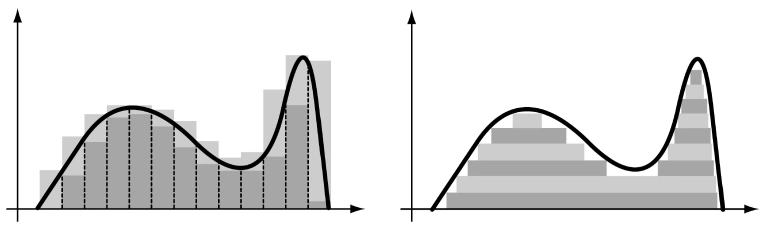
\includegraphics[width=0.75\linewidth]{img/riemann-vs-lebesgue.png}
 \vspace{0.5cm}
 \caption[Riemann and Lebesgue approximations]{Riemann and Lebesgue approximations \cite{schilling2017measures}}
 \label{figure:schilling}
\end{figure}

$$L_k^n=\{x\in\KK \,|\, t_k^n\le f(x)\le t_{k+1}^n\}.$$

Then the following approximation is usable for the area bounded by $f(D), y=0, x=a$ and $x=b$ for $D=[a,b]$, which coincides with Riemann integral.

\begin{equation}
 \label{example:lebesgue-partition}
 I_n=\sum\limits_{k=0}^{m_n-1}(t_{k+1}-t_k)\lambda(L_k^n).
\end{equation}

The additional requirement is that each $L^n_k$ is Lebesgue measurable. In Riemann integral, the function $f$ is required to be discontinuous at finite number of points, which is less general than Lebesgue measurability. Furthermore, Equation \ref{example:lebesgue-partition} can be generalized for abstract set $\Omega$ rather than $\RR^d$, its $\sigma$-algebra $\F$ and a measure $\mu$. In such measure space $(\Omega, \F, \mu)$, we will formally construct the Lebesgue integral for each measurable function $f:\Omega\to\RR$. The idea is to approximate $f$ by the limit of a sequence of steps function $(f_n)_{n\in\NN}$.

\begin{definition}[Step function]
 Let $(\Omega, \F, \mu)$ be a measure space. A function $f:\Omega\to\RR$ is a \textbf{step function}\index{step function} if there exists $\{A_n\}_{n=1}^N\subset\Omega$ and $\{c_n\}_{n=1}^N\subset\RR$ such that
 \begin{equation}
  f(x)=\sum\limits_{i=1}^nc_i\mathbf{1}_{A_i}(x).
 \end{equation}
\end{definition}

\begin{proposition}
 \label{proposition:standard-representation-of-a-step-function}
 Let $(\Omega, \F, \mu)$ be a measure space. Let $f:\Omega\to(0,\infty)$ be a positive step function. Then there exists a disjoint family $\{A_n\}_{n=1}^N\subset\Omega$ of nonempty sets, and a distinct set $\{c_n\}_{n=1}^N$ of positive number, such that
 \begin{equation}
  f(x)=\sum\limits_{n=1}^Nc_n\mathbf{1}_{A_n}(x).
 \end{equation}
 Moreover, this representation is unique.
\end{proposition}
\begin{proof}
 If there exist non-disjoint $A_i$ and $A_j$, we rewrite
 $$c_i\mathbf{1}_{A_i}(x) + c_j\mathbf{1}_{A_j}(x) = c_i\mathbf{1}_{A_i\setminus A_j}(x) + (c_i+c_j)\mathbf{1}_{A_i \cap A_j}(x) + c_j\mathbf{1}_{A_j\setminus A_i}(x),$$
 to achieve a disjoint family.

 If there exist $c_i = c_j$, we rewrite
 $$c_i\mathbf{1}_{A_i}(x) + c_j\mathbf{1}_{A_j}(x) = (c_i+c_j)\mathbf{1}_{A_i}(x) + c_j\mathbf{1}_{A_j\setminus A_i}(x).$$

 Then the attained subset of $\RR$ is disjoint. Let us abuse the original notation
 $$f(x)=\sum\limits_{n=1}^N c_n\mathbf{1}_{A_n}(x)$$
 for this new representation. For each $A_n, n\in\{1,\ldots,N\}$, choose $x_n\in A_n$. We have $f(x_n) = c_n > 0$. Now, consider two such representations
 $$f(x)=\sum\limits_{n=1}^Nc_n\mathbf{1}_{A_n}(x) = \sum\limits_{m=1}^Md_m\mathbf{1}_{B_m}(x).$$

 If $\bigcup_{n=1}^N A_n\setminus \bigcup_{m=1}^M B_m \ne \varnothing$, taking an element $x_0$ in this difference yields a contradiction when computing $f(x_0)$. Therefore, $\bigcup_{n=1}^N A_n\setminus \bigcup_{m=1}^M B_m = \varnothing$. Similar argument shows that $\bigcup_{n=1}^N A_n = \bigcup_{m=1}^M B_m$. Hence, for each $A_n, n\in\{1,\ldots, N\}$, there exists $B_m$ where $m\in\{1,\ldots,M\}$ such that $A_n\cap B_m\ne \varnothing$. Take $x_1\in A_n\cap B_m$, we have $f(x_1) = c_n = d_m$. If $A_n\setminus B_m \ne \varnothing$, take $x_2$ in this difference, then $f(x_2) = c_n = d_k$ for some $k\in\{1,\ldots,M\}$, a contradiction to the fact that $\{d_m\}$ is disjoint. Therefore, $A_n = B_m$. Thus, the representation is unique.
\end{proof}
\begin{remark}
 The representation in Proposition \ref{proposition:standard-representation-of-a-step-function} is called the standard representation. We can check that each positive step function $f$ has the standard representation
 \begin{equation}
  f(x) = \sum\limits_{t\in f(\Omega)} t\mathbf{1}_{\{x\in \Omega : f(x) = t\}}(x).
 \end{equation}
 If $f = 0, a.e.$, we choose the representation $f(x) = 0\cdot \mathbf{1}_{\Omega}(x)$. Let us denote by $\S^+$ the set of nonnegative step functions.
\end{remark}

\begin{corollary}
 Let $(\Omega, \F, \mu)$ be a measure space. Let $f:\Omega\to\RR$ be a step function. Then there exist a unique pair $f^+, f^-\in \S^+$ such that $f = f^+ - f^-$.
\end{corollary}

\begin{definition}[Lebesgue Integral of a Step Function]
 Let $(\Omega,\F,\mu)$ be a measure space and $f(x)=\sum\limits_{i=1}^nc_i\mathbf{1}_{A_i}(x)$ be a step function. The Lebesgue integral of $f$ with respect to a measure $\mu$ is defined as
 $$\int_\Omega f \d \mu = \sum\limits_{i=1}^nc_i\mu(A_i).$$
\end{definition}

We can see that the Lebesgue integral of a step function $f$ whose value coincides with the Riemann integral of $f$.

\begin{proposition}
 \label{proposition:integral-of-almost-everywhere-equal-step-functions}
 Let $(\Omega, \F, \mu)$ be a measure space and $f\in\S^+$. Suppose that $\Omega = E\cup E^c$, where $\mu(E^c) = 0$. Define a function $\tilde{f}:\Omega\to\RR$ as
 $$\tilde{f}(x) =\begin{cases}
   f(x), & \text{ if } x\in E    \\
   a,    & \text{ if } x\in E^c.
  \end{cases}$$
 Then $\int_\Omega f \d \mu = \int_\Omega \tilde{f} \d \mu$.
\end{proposition}

\begin{proof}
 We have
 \begin{align*}
  \int_\Omega \tilde{f} \d \mu
   & = \sum\limits_{t\in \tilde{f}(\Omega)} t\mu\left(\{x\in \Omega : \tilde{f}(x) = t\}\right)                                                                                                \\
   & = \sum\limits_{t\in \tilde{f}(\Omega)} t\mu\left(\{x\in E : \tilde{f}(x) = t\}\right) + \underbrace{a\mu(E^c)}_{0}                                                                        \\
   & = \sum\limits_{t\in \tilde{f}(\Omega)} t\mu\left(\{x\in E : \tilde{f}(x) = t\}\right)                                                                                                     \\
   & = \sum\limits_{t\in \tilde{f}(\Omega)} t\mu\left(\{x\in E : \tilde{f}(x) = t\}\right) + \underbrace{\sum\limits_{t\in \tilde{f}(\Omega)} t\mu\left(\{x\in E^c : \tilde{f}(x) = t\}\right)
  }_{0}                                                                                                                                                                                        \\
   & = \sum\limits_{t\in \tilde{f}(\Omega)} t\left[\mu\left(\{x\in E : \tilde{f}(x) = t\}\right) + \mu\left(\{x\in E^c : \tilde{f}(x) = t\}\right)\right]                                      \\
   & \sum\limits_{t\in \tilde{f}(\Omega)} t\mu\left(\{x\in \Omega : \tilde{f}(x) = t\}\right)                                                                                                  \\
   & = \int_\Omega f \d \mu.
 \end{align*}
\end{proof}

\begin{definition}
 Let $f:\Omega\to[0,\infty)$ be measurable. The Lebesgue integral of $f$ is defined as
 \begin{equation}
  \int_\Omega f\d \mu = \sup\left\{\int\limits h\d \mu(h) : h\in\S^+, h\le f\right\}.
 \end{equation}
\end{definition}

\begin{definition}
 Let $f:\Omega\to\RR$ be measurable. Define $f^+(x) = \sup(f,0)$ and $f^-(x) = \sup(-f,0)$. The Lebesgue integral of $f$ is defined as
 \begin{equation}
  \int_\Omega f\d \mu = \int_\Omega f^+\d \mu - \int(-f^-)\d \mu
 \end{equation}
 Then $f$ is said to be integrable or summable if $\int_\Omega f\d \mu<\infty$.
\end{definition}

\begin{definition}
 Let $f:\Omega\to\RR$ be measurable and $E \in \F$. The integral of $f$ over $E$ is defined as
 \begin{equation}
  \int_E f\d \mu = \int_\Omega f\mathbf{1}_E\d \mu.
 \end{equation}
\end{definition}

\begin{remark}
 When $(\Omega, \F, \mu) = (\RR^d, \B{(\RR^d)}, \lambda)$, Lebesgue integral coincides with Riemann integral. In such case, we simply write
 \begin{equation}
  \int_B f\d\lambda = \int_B f(x)\d x, B\in\B(\RR^d).
 \end{equation}
\end{remark}

\begin{proposition}
 \label{proposition:integral-of-le-everywhere-functions}
 Let $(\Omega,\F,\mu)$ be a measure space. Let $f$ and $g$ be measurable functions such that $f\le g, \mu-a.e.$ Then
 \begin{equation}
  \int_\Omega f\d \mu \le  \int_\Omega g\d \mu.
 \end{equation}
\end{proposition}

\begin{proof}
 If $f\le 0  \le g, \mu-a.e.$, we can use step functions approximation to prove that $\int_\Omega f\d \mu \le 0 \le  \int_\Omega g\d \mu$. If $f\le g\le 0$, we will prove that $0\le \int_\Omega -g\d \mu \le \int_\Omega -f\d \mu$. Hence, let us consider the case $ 0  \le f\le  g, \mu-a.e.$ Denote $E = \{x\in \Omega : f(x) \le g(x)\}$, we have $\mu(E^c) = 0$. For a step function $h\in S^+$, define $\tilde{h}$ similarly as in Proposition  \ref{proposition:integral-of-almost-everywhere-equal-step-functions}. We have
 \begin{align*}
  \int_\Omega f\d \mu
   & = \sup\left\{\int_\Omega f\d \mu : h\in \S^+, h\le f\right\}                                  \\
   & = \sup\left\{\int_\Omega f\d \mu : \tilde{h}\in \S^+, \tilde{h}\le f \text{ on } E\right\}    \\
   & \le  \sup\left\{\int_\Omega f\d \mu : \tilde{h}\in \S^+, \tilde{h}\le g \text{ on } E\right\} \\
   & =  \sup\left\{\int_\Omega f\d \mu : \tilde{h}\in \S^+, h\le g\right\}                         \\
   & =  \int_\Omega g\d \mu.
 \end{align*}
\end{proof}

\begin{corollary}
 \begin{enumerate}[label=(\roman*), ref=(\roman*)]
  \item []
  \item If $f = g, \mu-a.e.$, then $\int_\Omega f\d \mu =  \int_\Omega g\d \mu$.
  \item If $\int_\Omega |f|\d \mu = 0$, then $f=0,\mu-a.e.$
 \end{enumerate}
\end{corollary}

\begin{proof}
 For statement (i), we have $f\le g$ and $g\le f$, $\mu$-a.e. The conclusion follows directly from Proposition \ref{proposition:integral-of-le-everywhere-functions}. For statement (ii), let $E = \{x\in\Omega : |f(x)| = 0\}$, we have
 \begin{align*}
  0
   & = \int_\Omega |f|\d \mu                    \\
   & = \int_E |f|\d \mu + \int_{E^c} |f|\d \mu  \\
   & = \int_{E^c} |f|\d \mu                     \\
   & \ge \int_{E^c} \inf\limits_{E^c} |f|\d \mu \\
   & = \inf\limits_{E^c} |f| \mu (E^c)          \\
   & \ge 0
 \end{align*}
 Thus, $\mu (E^c)=0$ or $f=0$, $\mu$-a.e.
\end{proof}

To conclude this discussion of Lebesgue integral, we introduce $L^p$ spaces, crucial Banach spaces in functional analysis, particularly relevant for theorems in stochastic processes.

\begin{definition}
 \label{definition:Lp-space}
 Let $(\Omega,\F,\mu)$ be a measure space and $p\ge1$. The $L^p := L^p(\mu)$ space includes every function $f:\Omega\to\RR^m$, such that
 $$\left(\int\limits_\Omega \|f\|^p_p\d \mu\right)^{1/p}<\infty.$$
\end{definition}

\begin{remark}
 We can also define $L^\infty$ space. However, in the scope of the project, let us focus on $L^2$ onward. Those keen on delving deeper can refer to popular textbooks on Measure Theory \cite{cohn2013measure} or Functional Analysis \cite{rudin1987functional}.
\end{remark}

\begin{theorem}
 \label{theorem:L2-is-Banach}
 The $L^2$ space in Definition \ref{definition:Lp-space} is a vector space. The function $\|\cdot\|_{L^2} : L^2\to\RR$ be defined by
 $$\|f\|_{L^2(\mu)}=\left(\int\limits_\Omega \|f(x)\|^2_2\d \mu\right)^{1/2}, \forall f\in L^2.$$
 is a norm in the $L^2$ space. Moreover, the normed space $(L^2, \|\cdot\|_{L^2})$ is Banach.
\end{theorem}

\begin{proof}
 Firstly, we prove that $L^2$ is a vector space. Let $f,g \in L^2$, it is sufficient to show that $f+kg\in L^2$, for $k\in\RR$. Indeed, we have
 \begin{align*}
  \left(\int\limits_\Omega \|f + kg\|^2_2\d \mu\right)^{1/2}
   & \le \left(\int\limits_\Omega \left(\|f\|^2_2 + k^2\|g\|^2_2\right)\d \mu\right)^{1/2}                               \\
   & = \left(\int\limits_\Omega \|f\|^2_2\d \mu\right)^{1/2}  + \left(k^2\int\limits_\Omega \|g\|^2_2\d \mu\right)^{1/2} \\
   & < \infty.
 \end{align*}
 Now we prove that $\|\cdot\|_{L^2}$ is a norm. Nonnegativity and homogeneity are straightforward. Note that the function
 $\langle \cdot, \cdot\rangle : L^2 \times L^2\to \RR$ defined by
 \begin{equation}
  \langle f,g \rangle = \int\limits_\Omega fg \d \mu, \forall f,g\in L^2
 \end{equation}
 is a dot product in $L^2$. Using Cauchy-Schwarz inequality for any $f,g\in L^2$, we have
 \begin{align*}
  \|f + g\|_{L^2}^2
   & = \int\limits_\Omega \|f + g\|^2_2\d \mu                                                                                                                             \\
   & = \int\limits_\Omega (\|f\|_2 +\|g\|_2)^2\d \mu                                                                                                                      \\
   & = \int\limits_\Omega \|f\|_2^2\d \mu + \int\limits_\Omega \|g\|_2^2\d \mu + 2\int\limits_\Omega \|f\|_2\|g\|_2\d \mu                                                 \\
   & \le  \int\limits_\Omega \|f\|_2^2\d \mu + \int\limits_\Omega \|g\|_2^2\d \mu + 2\left(\int\limits_\Omega \|f\|_2\d \mu \int\limits_\Omega \|g\|_2\d \mu\right)^{1/2} \\
   & = \left( \left(\int\limits_\Omega \|f\|_2\d \mu\right)^{1/2} + \left(\int\limits_\Omega \|g\|_2\d \mu\right)^{1/2} \right)^2                                         \\
   & = \left(\|f\|_{L^2} + \|g\|_{L^2}\right)^2.
 \end{align*}
 Thus, triangle inequality is also satisfied.

 Finally, we prove that $L^2$ is complete. Consider a sequence $(f_n)_{n=1}^\infty\subset L^2$ such that $\lim\limits_{n\to\infty}\|f-f_n\|_{L^2}$. We have $\|f\|_{L^2}\le \|f-f_n\|_{L^2} + \|f_n\|_{L^2}, \forall n\in \NN$. Therefore,
 $$\|f\|_{L^2} \le \lim\limits_{n\to\infty}\left(\|f-f_n\|_{L^2} + \|f_n\|_{L^2}\right) = \lim\limits_{n\to\infty} \|f_n\|_{L^2} < \infty.$$
\end{proof}

